\documentclass[11pt,a4paper]{article}
\usepackage[a4paper, top=18mm, bottom=18mm, left=20mm, right=20mm]{geometry}
\usepackage{times}
\usepackage{amsmath}
\usepackage{amssymb}
\usepackage{graphicx}
\usepackage{float}
\usepackage{booktabs}
\usepackage{titlesec}
\usepackage{caption}

\titleformat{\section}{\normalfont\large\bfseries}{}{0em}{}
\titleformat{\subsection}{\normalfont\normalsize\bfseries\itshape}{}{0em}{}
\titlespacing{\section}{0pt}{8pt}{2pt}
\titlespacing{\subsection}{0pt}{5pt}{1pt}

\setlength{\parindent}{0pt}
\setlength{\parskip}{4pt}

\begin{document}

\begin{center}
{\fontsize{13}{15}\selectfont\textbf{%
Why Your Brain Goes Blank During Exams: A Dynamical Systems Proof}}

\vspace{8pt}

{\fontsize{13}{15}\selectfont\textbf{Parth Mehta}}\\[2pt]
{\fontsize{11}{13}\selectfont BITS Pilani, Pilani Campus}\\[2pt]
{\fontsize{11}{13}\selectfont parth@example.com}
\end{center}

\vspace{5pt}\hrule\vspace{5pt}

\section*{Abstract}

You studied, you revised, you even made colour-coded notes. And then,
mid-exam, the moment the invigilator says "you may begin now" - nothing. Your mind, a
perfectly organised library five minutes ago, is now an empty car park.

This paper proves that this is not your fault. Using three coupled
nonlinear differential equations, we model the exam blackout as a
\emph{working memory hijacking}: stress generates anxious rumination
that physically crowds recall out of your finite cognitive workspace.
The model reproduces the Yerkes-Dodson inverted-U, the cascade
triggered by a single hard question, and the infuriating post-exam
clarity that hits the moment you walk out the door. We derive a
closed-form bound on blackout severity and three mathematically
grounded escape routes.

\vspace{4pt}\hrule\vspace{6pt}

\section{Introduction}

Every student on the planet has experienced this: spend days
preparing, sit down to write, then watch in silent horror as
everything vanishes into a cognitive black hole. The standard
explanation - ``you were just anxious'' is about as useful as
telling someone drowning that the problem is being in too much water (We should add this to the words of wisdom).
It does not explain why the collapse is sudden, why thinking harder
makes it worse, or why it ends the instant the invigilator says
``pens down.''

The aim of this paper is to prove with actual mathematics that
the exam blackout is a \emph{deterministic trajectory in a nonlinear
dynamical system}, driven by a positive feedback loop between stress
and rumination that hijacks working memory. The obvious fact we are
proving: \emph{a very hard exam question can make you forget
everything, even material you definitely know.} The less obvious
part: \emph{this follows inevitably from three differential equations,
and the timing of recovery is equally predictable.}

\section{Body}

\subsection{The Variables}

\textbf{$S(t) \geq 0$: Stress.} Zero at breakfast. Considerably
higher when you flip to question 2.

\textbf{$R(t) \in [0,1]$: Recall efficiency.} At 1.0, you are the
student everyone hates. At 0, you are producing nothing but a slowly
spreading sense of existential dread.

\textbf{$L(t) \in [0,1]$: Rumination load.} The fraction of working
memory occupied by intrusive thoughts - ``everyone else is writing,''
``I am going to fail,'' ``what if I become a 'worm'.'' At $L=1$,
there is literally no cognitive space left for chemistry.

Working memory capacity $W(S)$ shrinks with stress:
\begin{equation}
  W(S) = \frac{1}{1 + k_w S}
  \label{eq:W}
\end{equation}
Full capacity at zero stress. Increasingly useless as the clock ticks.

\subsection{The Three Equations of Doom}

\textbf{Stress:}
\begin{equation}
  \dot{S} = \alpha T(t) - \beta S - \gamma R - \mu E
  \label{eq:S}
\end{equation}
Stress grows with time pressure $T(t)$, decays naturally at rate
$\beta$, drops when you successfully recall things, and is biased
upward by poor exam history ($E < 0$). The time pressure profile
rises linearly during the exam and drops discontinuously to zero
the moment it ends, a fact that  will become important shortly.

\textbf{Recall:}
\begin{equation}
  \dot{R} = \frac{\rho}{1 + k_w S}(1-L)(1-R) - \delta R
  \label{eq:R}
\end{equation}
Your recall rate is gated by working memory capacity $W(S)$,
the fraction of working memory not already consumed by rumination
$(1-L)$, and logistic saturation. This single equation produces
the Yerkes-Dodson inverted-U automatically, no parameter tuning is
required.

\textbf{Rumination:}
\begin{equation}
  \dot{L} = \sigma S(1-L) - \tau R L - \nu L
  \label{eq:L}
\end{equation}
Stress fills working memory with anxious thoughts. Successful recall
actively evicts those thoughts, answering a question correctly
literally suppresses the worried ruminations competing for the same
mental space. Rumination also decays passively at rate $\nu$ when
nothing is driving it.

\subsection{The Toggle Switch}

Look at Equations~(\ref{eq:R}) and~(\ref{eq:L}) together. High $R$
drives $-\tau RL$ strongly negative, suppressing $L$. High $L$
shrinks $(1-L)$ in Eq.~(\ref{eq:R}), suppressing $R$. Each variable
suppresses the other, a \emph{mutual inhibition loop}, the same
topology as a biological toggle switch or a flip-flop circuit.
The system has two stable states and snaps between them:

\begin{center}
\begin{tabular}{lcc}
\toprule
\textbf{State} & \textbf{Recall $R$} & \textbf{Rumination $L$} \\
\midrule
Functional (flow) & High & Low \\
Blackout          & Low  & High \\
\bottomrule
\end{tabular}
\end{center}

\subsection{Stability: Why the Functional State Holds (Until It Doesn't)}

To prove the functional state is stable, we linearise the system
around the fixed point $(S_F, R_F, L_F)$ and compute the Jacobian:
\begin{equation}
  J =
  \begin{pmatrix}
    -\beta & -\gamma & 0 \\[3pt]
    \partial_S\dot{R} & -\rho W(1-L)-\delta & -\rho W(1-R) \\[3pt]
    \sigma(1-L) & -\tau L & -\sigma S-\tau R-\nu
  \end{pmatrix}
  \label{eq:J}
\end{equation}
where $\partial_S\dot{R} = -k_w\rho(1-L)(1-R)/(1+k_wS)^2$.
The key entries are $J_{23} = -\rho W(1-R) < 0$ and
$J_{32} = -\tau L < 0$: the mutual suppression pair. Their product
$J_{23} \cdot J_{32} = \tau L \rho W(1-R) > 0$ contributes
positively to the determinant, which is the Routh-Hurwitz
requirement for a stable fixed point.

Numerically, the eigenvalues at the functional fixed point for
mid-exam pressure ($T = 0.65$) are:
\begin{equation}
  \lambda \in \{-0.268,\;\; -2.121 \pm 0.271i\}
  \label{eq:eigs}
\end{equation}
All real parts are strictly negative: the functional state is a
\emph{locally stable spiral}. Perturbations decay back to it in
damped oscillations. Your brain actively resists the blackout.

The instability is not in the fixed point, it is in the
\emph{basin of attraction}. As exam pressure $T$ increases, the
fixed point remains stable, but the basin shrinks: the Jacobian
entries $J_{23}$ and $J_{32}$ weaken as $W(S)$ degrades and $L$
drifts higher, reducing the product $J_{23}\cdot J_{32}$ and
narrowing the margin around the fixed point. A perturbation that
would have decayed harmlessly early in the exam can, late in the
exam, kick the trajectory past the basin boundary, after which
the nonlinear dynamics take over and drive the system to the
blackout state regardless of effort. The functional fixed point
never became unstable. The neighbourhood of safety around it
simply became too small.



\begin{figure}[H]
  \centering
  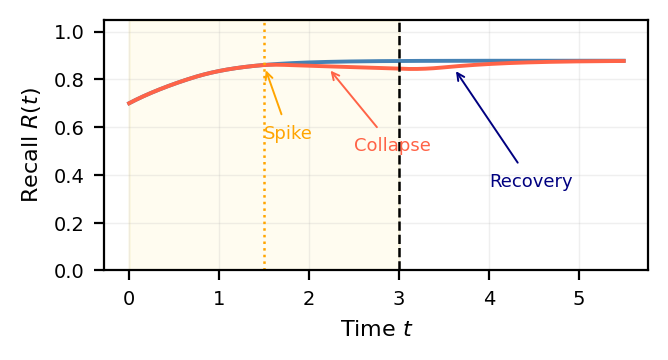
\includegraphics[width=0.62\textwidth]{figures_psych/bk_R.png}
  \caption{Recall $R(t)$. Blue: manageable exam. Red: stress spike at
  $t=1.5$ (one hard question). Collapse is immediate; post-exam
  recovery is sharp and total. The information was never lost---the
  pipeline was hijacked.}
  \label{fig:bk_R}
\end{figure}



\subsection{Post-Exam Clarity: The Most Annoying Theorem in This Paper}

When the exam ends, $T$ drops to zero. The stress source vanishes.
$S$ decays, the rumination source $\sigma S(1-L)$ disappears, $L$
decays via $-\nu L$, working memory clears, and $R$ recovers, 
self-reinforced by the mutual inhibition loop. The information was
in long-term memory the entire time. This is why you remember the
answer to question 4 on your way to mess. The math demanded it.

\subsection{Why Exam History Is a Parameter}

The term $-\mu E$ in Eq.~(\ref{eq:S}) means a student with a history
of failure ($E<0$) starts every exam already displaced toward the
blackout regime. A student starting with higher baseline stress needs a smaller perturbation
to tip the trajectory into the blackout basin. Same exam. Same equations. Different $E$.

\begin{figure}[H]
  \centering
  \begin{minipage}{0.48\textwidth}
    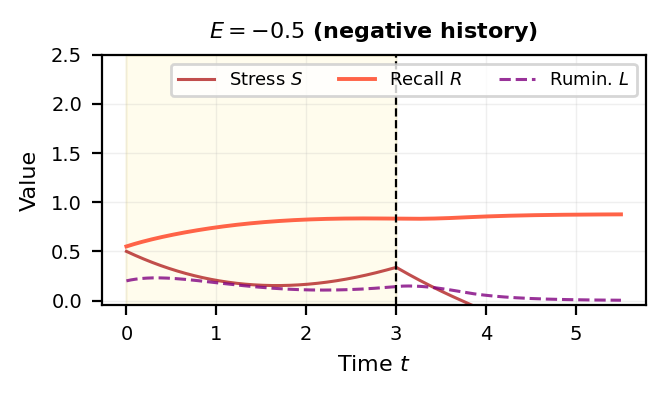
\includegraphics[width=\textwidth]{figures_psych/prior_neg.png}
    \caption*{$E=-0.5$: rumination saturates, recall collapses.}
  \end{minipage}\hfill
  \begin{minipage}{0.48\textwidth}
    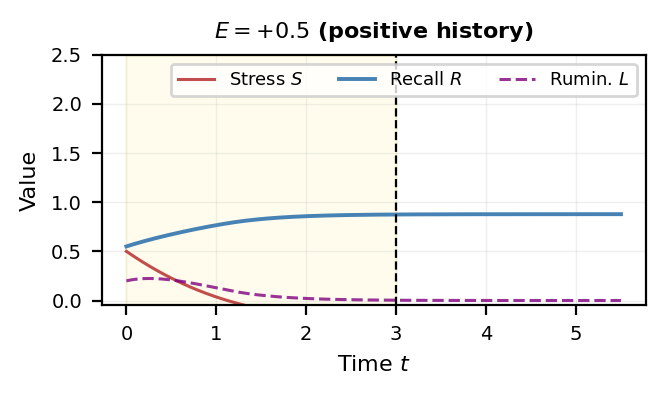
\includegraphics[width=\textwidth]{figures_psych/prior_pos.png}
    \caption*{$E=+0.5$: barely any rumination. Same exam.}
  \end{minipage}
  \caption{Effect of prior exam history $E$ on the same exam.
  Left: negative history. Right: positive history.}
  \label{fig:prior}
\end{figure}

\subsection{Three Escape Routes, With Proof}

\textbf{Write anything.} In the blackout state $R \approx 0$ and
the $-\tau RL$ suppression of rumination has vanished. Write down
anything, even if it's wrong. This inserts a non-zero $R$, immediately
reactivating $-\tau RL$, driving $L$ down, clearing working memory,
and initiating recall recovery. The content need not be correct.
This is not advice. This is a theorem: reactivating the mutual suppression
term $-\tau RL$ reverses the cascade.

\textbf{Actually breathe.} Controlled breathing raises the physiological
stress decay rate $\beta$ in Eq.~(\ref{eq:S}), accelerating the removal of
the rumination source $\sigma S(1-L)$. Mindfulness raises the passive
rumination decay $\nu$ in Eq.~(\ref{eq:L}). Both speed recovery.
The maths does not care whether you believe in mindfulness; it cares about $\nu$.

\textbf{Reframe your history.} Shifting $E$ toward positive values via
cognitive reframing lowers the baseline stress $S_F(T)$ from which every
exam begins, widening the basin of the functional state and requiring
larger perturbations to trigger the blackout cascade.



\section{Conclusion}

The exam blackout is a cascade in a mutual inhibition system.
Stress generates rumination, rumination occupies working memory,
reduced working memory lowers recall, reduced recall weakens the
suppression of rumination, which generates more rumination.
The loop closes. The system tips. You forget your own name.

The information was never gone. Three interventions derived directly
from the governing equations can interrupt or prevent the cascade. None of this makes
exams less stressful. But the next time your mind goes blank,
you can at least comfort yourself that you are not failing, you
are experiencing an attractor bifurcation. Mathematically rigorous
cold comfort is still cold comfort, but it is of the best kind.

\section*{Appendix}

\subsection*{Parameter Values} \vspace{-4pt}

\begin{center}
\begin{tabular}{clc}
\toprule
\textbf{Param.} & \textbf{Meaning} & \textbf{Value} \\
\midrule
$\alpha$ & Time-pressure sensitivity    & 0.8  \\
$\beta$  & Stress decay rate            & 0.4  \\
$\gamma$ & Recall $\to$ stress relief   & 0.6  \\
$\mu$    & Prior performance weight     & 0.2  \\
$\rho$   & Max recall rate              & 1.8  \\
$k_w$    & WM stress sensitivity        & 1.0  \\
$\delta$ & Recall fatigue rate          & 0.25 \\
$\sigma$ & Stress $\to$ rumination rate & 1.2  \\
$\tau$   & Recall $\to$ rumin.\ suppression & 1.8  \\
$\nu$    & Passive rumination decay     & 0.35 \\
\bottomrule
\end{tabular}
\end{center}

\subsection*{Simulation}

Python 3, \texttt{scipy.integrate.solve\_ivp}, RK45,
\texttt{max\_step}$=0.005$. Source: \texttt{gen\_split\_figures.py}.

\end{document}